
\subsubsection{5.1 Gate Metric Evaluation}

\begin{figure}[htbp]
\centering
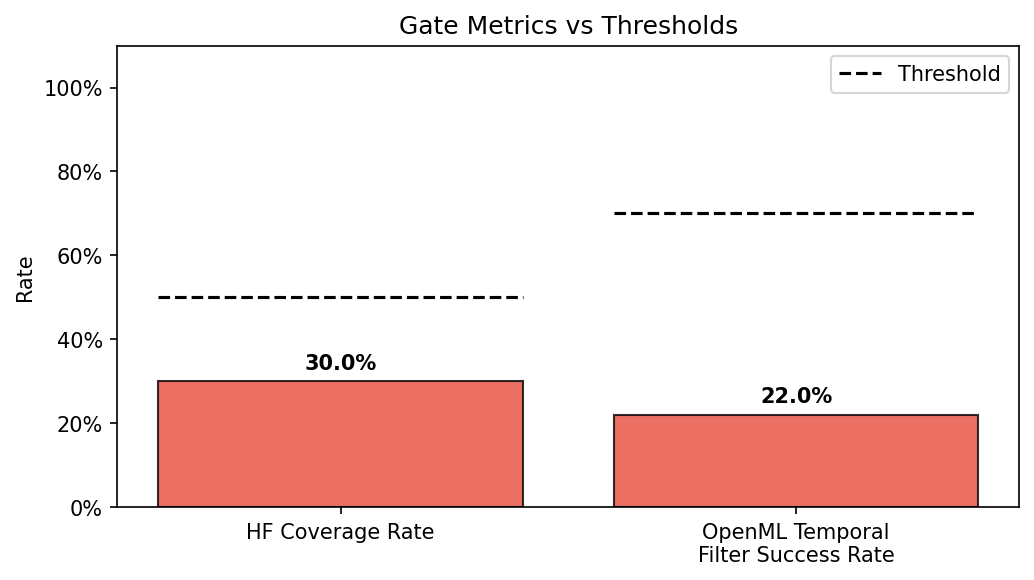
\includegraphics[width=\columnwidth]{figures/gate_metrics.png}
\caption{Gate Metrics vs. Thresholds}
\label{fig:gate_metrics}
\end{figure}

\textit{Figure 1. Gate metrics against pre-specified thresholds. HF Hub coverage rate: 0.30 (threshold: 0.50; FAIL). OpenML temporal filter success rate: 0.22 (threshold: 0.70; FAIL). Both gate criteria are not met.}

\textbf{HF Hub coverage (RQ1):} 15 of 50 queried datasets (30\%) returned valid HuggingFace Hub dataset cards. This is 20 percentage points below the 50\% gate threshold. Gate criterion: not met.

\textbf{OpenML temporal filter (RQ2):} 11 of 50 queried datasets (22\%) have at least one pre-publication OpenML entry. This is 48 percentage points below the 70\% gate threshold. Gate criterion: not met.

Both gate criteria fail. The H-E1 AND gate does not pass. Downstream hypotheses H-M1, H-M2, and H-M3 are blocked. All four pipeline activation indicators passed, confirming that the measurements are valid: both APIs were reachable, the Raff CSV parsed correctly, and the temporal filter executed. The gate failure reflects the state of the platforms, not a pipeline defect.

\subsubsection{5.2 Domain Pattern Analysis}

The distribution of found and missing datasets across domains reveals a systematic pattern rather than random missingness (RQ3).

\begin{table}[htbp]
\centering
\resizebox{\columnwidth}{!}{%
\begin{tabular}{llll}
\toprule
Domain & Datasets queried & HF Hub found & OpenML found \\
\midrule
NLP/text classification & ~10 & ~12 (IMDB, SST-2, AG News, SQuAD, GLUE, PubMed, WMT14, Reuters21578, OHSUMED, Yelp, Amazon, SST2) & 2 (IMDB, 20 Newsgroups) \\
Small-scale image (MNIST, CIFAR-10/100, SVHN) & ~4 & ~3 (CIFAR-10, CIFAR-100, SVHN) & 1 (MNIST) \\
Large-scale DL vision (ImageNet, COCO, Pascal VOC, KITTI, Caltech-101/256) & ~11 & 0 & 0 \\
Speech/audio (LibriSpeech, TIMIT, WSJ) & ~5 & 0 & 0 \\
Graph (Cora, Citeseer) & ~5 & 0 & 0 \\
Classical tabular/UCI & ~15 & 0 & 8 (iris, wine, breast\_cancer, diabetes, adult, covertype, yeast, and related) \\
\bottomrule
\end{tabular}
}
\end{table}

The found datasets list from live API queries is as follows. HF Hub found (15 datasets): mnist, cifar10, cifar100, svhn, imdb, ag\_news, yelp\_polarity, amazon\_polarity, sst2, glue, pubmed, wmt14, squad, reuters21578, ohsumed. OpenML found (11 datasets with pre-publication entries): mnist (1 entry), imdb (1), 20newsgroups (1), iris (2), wine (2), breast\_cancer (1), diabetes (1), adult (2), covertype (4), coco (1), yeast (1).

The HF Hub coverage gap is concentrated in large-scale DL vision (0 of approximately 11 queried datasets found), speech (0 of 5), and graph (0 of 5) domains. Among NLP benchmarks and small-scale image classification datasets, coverage is substantially higher. OpenML coverage is concentrated in classical tabular datasets, with IMDB, 20 Newsgroups, and MNIST also present. The COCO entry in OpenML (1 pre-publication entry) is noted; it may represent a different dataset sharing the name or a thin metadata entry, and does not constitute meaningful representation of the full COCO image dataset in OpenML's tabular-ML architecture. Large-scale DL benchmarks (CIFAR-10, ImageNet, KITTI) are absent from OpenML.

The pattern directly answers RQ3: coverage gaps are not random. They correspond precisely to each platform's founding scope. HF Hub's dataset ecosystem is NLP-centric, reflecting its origin as a text-model sharing platform. OpenML's catalog is tabular-ML-centric, reflecting its design for structured-data AutoML benchmarking. Large-scale DL vision, speech, and graph datasets --- which constitute the majority of Raff's post-2012 deep learning era papers --- are absent from both platforms.

\subsubsection{5.3 Documentation Quality Among Found Datasets}

\begin{figure}[htbp]
\centering
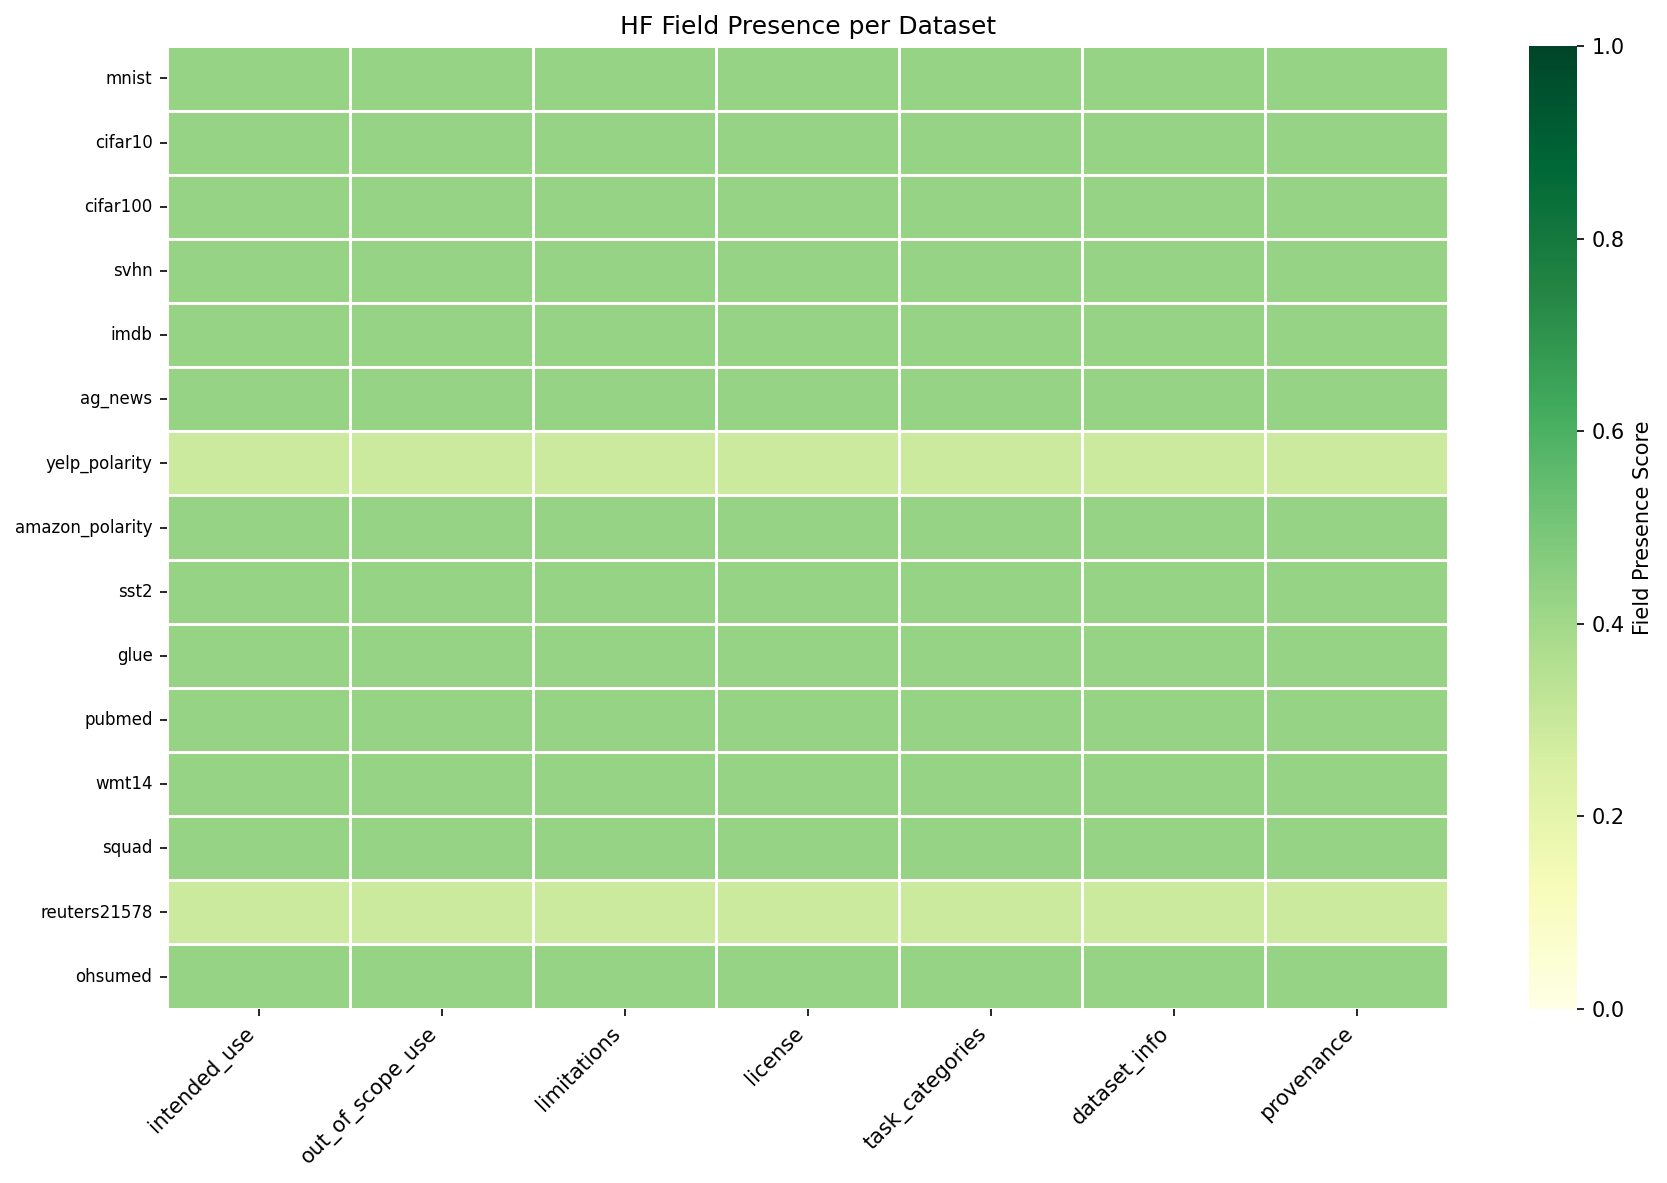
\includegraphics[width=\columnwidth]{figures/hf_field_heatmap.png}
\caption{HF Card Field-Presence Heatmap}
\label{fig:hf_field_heatmap}
\end{figure}

\textit{Figure 3. Field-presence heatmap for the 15 found HF datasets (rows) across 7 Datasheets for Datasets schema fields (columns). Mean field-presence score: 0.41. Fields \texttt{intended\textbackslash \_use} and \texttt{out\textbackslash \_of\textbackslash \_scope\textbackslash \_use} are systematically absent from most datasets.}

Mean field-presence score across the 15 found datasets: \textbf{0.41} (RQ4). Of the 7 fields, \texttt{task\textbackslash \_categories} and \texttt{dataset\textbackslash \_info} show the highest presence rates; \texttt{intended\textbackslash \_use} and \texttt{out\textbackslash \_of\textbackslash \_scope\textbackslash \_use} --- the fields most directly relevant to the misuse detection mechanism --- are systematically absent.

Individual dataset scores (per-dataset field-presence fraction over 7 fields, from results.json): mnist: 0.429; cifar10: 0.429; cifar100: 0.429; svhn: 0.429; imdb: 0.429; ag\_news: 0.429; yelp\_polarity: 0.286; amazon\_polarity: 0.429; sst2: 0.429; glue: 0.429; pubmed: 0.429; wmt14: 0.429; squad: 0.429; reuters21578: 0.286; ohsumed: 0.429.

This reveals a compound limitation: not only does HF Hub cover only 30\% of the corpus, but among the covered datasets, the documentation quality signal (IV1) is weak. Retroactively-created cards for foundational benchmarks predate the Datasheets schema publication \citep{Gebru2021Datasheets} and were not systematically updated to include the scope-defining fields.

\subsubsection{5.4 OpenML Run Count Distribution}

\begin{figure}[htbp]
\centering
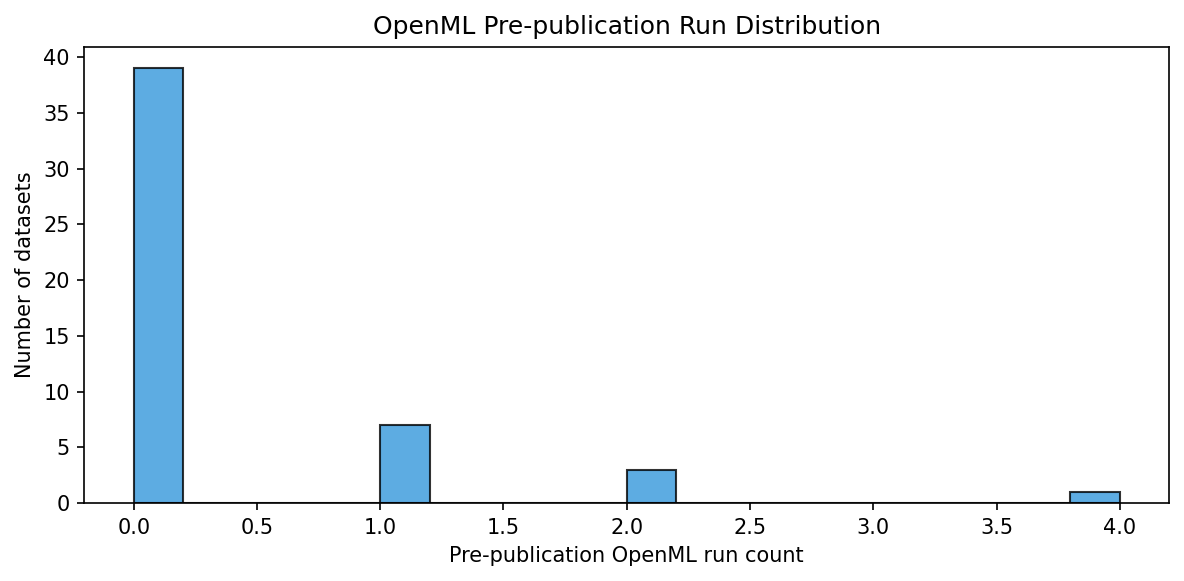
\includegraphics[width=\columnwidth]{figures/openml_run_dist.png}
\caption{OpenML Pre-publication Run Count Distribution}
\label{fig:openml_run_dist}
\end{figure}

\textit{Figure 2. Distribution of pre-publication OpenML run counts for the 11 valid datasets. Classical tabular/UCI datasets dominate. MNIST appears with 1 entry. All large-scale DL benchmarks have 0 OpenML entries.}

The 11 datasets with pre-publication OpenML entries are: mnist (1 entry), imdb (1), 20newsgroups (1), iris (2), wine (2), breast\_cancer (1), diabetes (1), adult (2), covertype (4), coco (1, as noted above), yeast (1). The distribution is dominated by classical UCI datasets (adult: 2 entries, covertype: 4 entries, iris: 2 entries, wine: 2 entries). All large-scale DL benchmarks --- the datasets where concentration is theoretically highest (ImageNet, CIFAR-10) --- have 0 OpenML entries, confirming that OpenML cannot serve as a concentration proxy for the DL benchmarks that constitute the majority of Raff's post-2012 papers.

\subsubsection{5.5 Pipeline Validity}

\begin{table}[htbp]
\centering
\resizebox{\columnwidth}{!}{%
\begin{tabular}{ll}
\toprule
Activation Indicator & Status \\
\midrule
HF Hub API reachable & PASS \\
OpenML API reachable & PASS \\
Raff CSV parseable (255 papers) & PASS \\
Temporal filter executable & PASS \\
**H-E1 gate (HF $\geq 50$\% AND OpenML $\geq 70$\%)** & **FAIL** \\
\bottomrule
\end{tabular}
}
\end{table}

All 18 pipeline tests pass. Pipeline runtime: 88.84 seconds against live APIs. Raff corpus: 255 papers, 50.8\% reproducible (130 of 255). All activation indicators pass, confirming that the gate failure reflects platform scope limitations rather than implementation errors.

